% !TeX encoding = UTF-8 Unicode
% !TEX root = MaksimenkoThesis.tex
%%%%%%%%%%%%%%%%%%%%%%%%%%%%%%%%%%%%%%%%%%%%%%%%%%%%%%%%%
%
%     Многогранники задач
%
%%%%%%%%%%%%%%%%%%%%%%%%%%%%%%%%%%%%%%%%%%%%%%%%%%%%%%%%%

\chapter{Многогранники задач}
\label{chap:Polytopes}
%\begin{flushright}
%При изучении наук примеры полезнее правил\\ \emph{И.~Ньютон}
%\end{flushright}

Основная цель этой главы "--- обзор известных результатов по теме диссертации.
Глава начинается с введения понятия семейства многогранников (полиэдров) задачи.
В~разделе~\ref{sec:Ident} обсуждается задача идентификации граней многогранников задач. В~разделе~\ref{sec:PolyhedralGraph} перечислены некоторые известные факты для таких полиэдральных характеристик задач, как число вершин, диаметр и кликовое число графа многогранника.
В~разделе~\ref{sec:ExtensionsAndRC} вводятся понятия расширения многогранника, его сложности и числа прямоугольного покрытия матрицы инциденций вершин"=гиперграней. В~разделе~\ref{sec:questions} формулируются общие вопросы, ответы на которые будут представлены в последующих главах.

\section{Многогранники и полиэдры задач}
\label{sec:ProblemPolytopes}

Обратим внимание на то, что индивидуальная линейная задача комбинаторной оптимизации по сути сводится к оптимизации линейной целевой функции $f(\bm{x}) = \bm{c}^T \bm{x}$ на некотором конечном множестве допустимых решений $X \in \Z^d$.
%(В~частности, $X$ является подмножеством вершин куба $\Cube_d$ в широко распространенном случае, когда $S = \{0,1\}$.)
Причем оптимальное значение целевой функции инвариантно относительно замены множества $X$ его выпуклой оболочкой $\conv(X)$.
Таким образом, линейная задача комбинаторной оптимизации эквивалентна оптимизации линейной функции на выпуклом многограннике $\conv(X)$.
%, называемом \emph{многогранником задачи}.
%Заметим, что один и тот же многогранник соответствует множеству индивидуальных задач, отличающихся друг от друга только целевыми векторами.
%\emph{Кодом} такого многогранника далее будем называть код $I$ соответствующей индивидуальной задачи, определяющий множество $X = X(I)$.
%, которая определяет множество допустимых решений $X$ (то есть не содержит избыточной информации о целевом векторе).
При такой интерпретации массовая задача ассоциируется с семейством многогранников.
В частности, в работе~\cite{Papadimitriou:1984}
предлагается формализовать задачу комбинаторной оптимизации как последовательность 0/1"~многогранников $\{P_n \mid n\in\N\}$ таких,
что для любого вектора $\bm{v}$ и индекса $n$ (кода многогранника)
мы можем за полиномиальное время проверить,
является ли $\bm{v}$ вершиной многогранника $P_n$.


\begin{definition}\label{def:family}
	Каждой линейной задаче комбинаторной оптимизации $(L, d, g)$ %(направление оптимизации может быть любым) 
	соответствует \emph{комбинаторное семейство многогранников} $\Set{P(I)\given I\in L}$, где многогранник $P(I)$ представляет собой выпуклую оболочку множества $X(I)$ из определения~\ref{def:LCOP}.
%	\[
%	X(I) = \Set*{\bm{x}\in\Z^d \given \size(\|\bm{x}\|_{\infty}) = \poly(\size(I)) \text{ и } g(\bm{x}, I)}.
%	\]
	Будем говорить, что семейство $\Set{P(I)\given I\in L}$ \emph{определяется тройкой $(L, d, g)$}, а $I \in L$ будем называть \emph{кодом} многогранника $P(I)$.
\end{definition}

\begin{remark}
Здесь и далее при определении специальных многогранников мы часто будем называть многогранником множество его вершин, подразумевая V"~описание многогранника.
Эта произвольность связана с тем, что нас, в первую очередь, будут интересовать две операции над многогранниками: аффинное отображение и пересечение с опорной гиперплоскостью. Результатом каждой из этих операций является выпуклый многогранник, причем множество вершин этого многогранника является результатом применения этих операций к множеству вершин исходного многогранника.
\end{remark}

\begin{comment}
\begin{remark}
Выбор пространства $\{0,1,\dots,k\}^d$ вместо более общего $\{a,a+1,\dots,b\}^d$, $a,b\in\Z$, объясняется тем, что любое множество $X \subseteq \{a,a+1,\dots,b\}^d$ элементарным смещением $\bm{x} \mapsto \bm{x} - \bm{a}$ преобразуется в множество $X' \subseteq \{0, k\}^d$, где $k = b-a$.
При этом не меняются не только комбинаторно"=геометрические свойства этого множества, но и сложность задачи линейной оптимизации на нем.
(Предполагается, что $a$ и $b$, также, как и $k$ в определении~\ref{def:family}, полиномиально вычислимы относительно кода многогранника.)
\end{remark}
\end{comment}
\begin{remark} 
В~\cite[с.~420]{ZieglerBook} комбинаторным многогранником называется класс комбинаторно эквивалентных выпуклых многогранников.
В~\cite{Naddef:1981, MatsuiTamura:1995} комбинаторными называются многогранники, у которых для каждой пары несмежных вершин середина соединяющего их отрезка является также серединой отрезка, соединяющего (некоторую) другую пару вершин этого многогранника.
В~настоящей работе эти определения не используются.
\end{remark}

\begin{remark}
\label{def:Psize}
Обратим внимание на тот факт, что свойства многогранника $X(I)$ никак не зависят от значений координат целевого вектора $\bm{c}$ соответствующей задачи $(L, d, g)$.
Это согласуется с тем, что во многих случаях сложность алгоритмов для задач такого типа оценивается числом арифметических операций и операций сравнения и не зависит от размера $\size(\bm{c})$ (не путать с размерностью). Так, например, сложность алгоритма Дейкстры для нахождения кратчайшего пути в полном графе обычно полагается равной $O(n^2)$, а алгоритм Хелда--Карпа решает задачу коммивояжера за время $O(n^2 2^n)$ (в обоих случаях размеры длин ребер графа игнорируются). В связи с этим, далее будем оценивать сложность задачи $(L, d, g)$ относительно величины $\size(I) + d(I)$, называемой \emph{размером} задачи или \emph{размером} многогранника $X(I)$. То есть будем предполагать, что умножение, сложение и сравнение чисел выполняются за единицу времени.
%Суммарная длина аргументов предиката $g$ равна $d \cdot \poly(\size(I) + d) + \size(I)$, то есть полиномиальна относительно суммы $d + \size(I)$, называемой в главах \ref{chap:AffTheory}--\ref{chap:ExtAff} \emph{размером многогранника} $X(I)$.
\end{remark}

Обратимся к примерам.

С задачей булева квадратичного программирования ассоциируется \emph{булев квадратичный многогранник}
\begin{equation}
\label{eq:BQP}
\BQP(n) = \Set*{\bm{x}=(x_{ij}) \in \{0, 1\}^{n(n+1)/2} \given x_{ij} = x_{ii} x_{jj}, \ 1 \le i < j \le n},
\end{equation}
обладающий многими интересными свойствами~\cite{Deza:2001}.
В данном случае параметр $n \in \N$ является кодом многогранника.

Булев квадратичный многогранник тесно связан с \emph{многогранником разрезов}{\label{def:CutPolytope}} $\Cut(n) \subseteq \R^{n(n-1)/2}$, вершинами которого являются характеристические вектора разрезов полного неориентированного графа на $n$ вершинах~\cite{Deza:2001}.

С задачей отыскания максимума многочлена на множестве целых точек отрезка $[a, b]$ связан циклический многогранник
\begin{equation}
\label{eq:Cyclic}
\CP_d(a,b) = \Set*{(x, x^2, \dots, x^d) \given \ a \le x \le b, \ x\in \Z}.
\end{equation}
Здесь кодом многогранника служит тройка $(d,a,b)$.

\emph{Многогранник задачи о рюкзаке} представляет собой выпуклую оболочку подмножества 0/1-векторов,
%вершин гиперкуба $\Cube_d$, 
принадлежащих полупространству $H^-(\bm{a}, b)$, $\bm{a} = (a_i) \in \Z^n$, $b \in \Z$:
\begin{equation}
\label{eq:KNAP}
\Knap(\bm{a},b) = \Set*{\bm{x} \in \{0,1\}^{n} \given \bm{a}^T \bm{x} \le b}.
\end{equation}
Кодом многогранника является пара $(\bm{a},b)$.

\hypertarget{def:PathPolytope}{Пусть} $G(V,E)$ "--- полный неориентированный граф на $n$ ($n=|V|$) вершинах, среди которых выделены две: $s$ и $t$.
Пусть $W \subseteq 2^E$ "--- множество всех $s$-$t$ путей в этом графе.
\emph{Многогранником путей} называется выпуклая оболочка множества всех характеристических векторов $\Path(n) \subseteq \{0,1\}^E$ для путей из $W$.
Аналогично определяется \emph{многогранник орпутей} $\Dipath(n) \subseteq \{0,1\}^A$ для полного ориентированного графа $D(V,A)$ на $n$ вершинах.

С многогранником путей тесно связан \emph{многогранник задачи коммивояжера} или
\label{def:TSP}
\emph{многогранник гамильтоновых циклов} %~\cite{Emelichev:1981} 
$\TSP(n)$, представляющий собой выпуклую оболочку множества характеристических векторов всех гамильтоновых циклов полного неориентированного графа на $n$ вершинах.
В свою очередь, выпуклая оболочка множества характеристических векторов гамильтоновых контуров в полном ориентированном графе на $n$ вершинах называется \emph{многогранником асимметричной задачи коммивояжера} или \emph{многогранником гамильтоновых контуров} и обозначается $\ATSP(n)$.

Задаче о сортировке массива (по-видимому, одной из самых востребованных на практике) соответствует семейство \emph{перестановочных многогранников}~\cite{Emelichev:1981} или \emph{пермутоэдров}~\cite{ZieglerBook}.\label{def:perm-birk}
Вершинами пермутоэдра $\Perm(n)$ являются вектора,
полученные всевозможными перестановками координат вектора $(1, 2, \dots, n)$.
Если же для перестановки $\pi \from [n] \to [n]$
вместо вектора $(\pi(1), \pi(2), \dots, \pi(n))$
мы рассмотрим перестановочную матрицу $\bm{x} \in \{0,1\}^{n\times n}$ с компонентами
\[
x_{ij} = \begin{cases}
1,& \text{если $\pi(i) = j$,}\\
0& \text{иначе,}
\end{cases}
\]
то получим \emph{многогранник Биркгофа} $\Birk(n)$, который еще называется \emph{многогранником бистохастических матриц} и \emph{многогранником задачи о назначениях}~\cite{Emelichev:1981}.
Перестановочную матрицу $\bm{x}$ можно также интерпретировать как характеристический вектор совершенного паросочетания в полном двудольном графе,
каждая доля которого содержит по $n$ вершин. 
С этой точки зрения многогранник $\Birk(n)$ может быть также назван многогранником совершенных паросочетаний в двудольном графе.

\emph{Многогранник совершенных паросочетаний} $\Match(n)$ определяется как выпуклая оболочка всех характеристических векторов совершенных паросочетаний в полном графе на $n$ вершинах.

Задача о поиске в полном реберно"=взвешенном графе $G(V,E)$ минимального (по суммарному весу входящих ребер) остовного (то есть связывающего все вершины графа) дерева может быть переформулирована как задача оптимизации на \emph{многограннике остовных деревьев} $\Tree(n) \subset \{0,1\}^{E}$, $n = |V|$, вершинами которого являются характеристические векторы остовных деревьев в графе~$G$.

Обобщением многогранников остовных деревьев являются многогранники матроидов (точнее, баз матроидов). 
В~\cite{Feichtner:2005} приводится весьма оригинальное, но вместе с тем краткое и емкое определение этих многогранников.
0/1"~многогранник в $\R^n$ называется \emph{многогранником матроида}, если он лежит в гиперплоскости $H(\bm{1}, r)$ при некотором целом $r \in [n]$ и его вершины удовлетворяют следующему критерию смежности\label{matroid}: вершины $\bm{x}$ и $\bm{y}$ смежны тогда и только тогда, когда найдутся $i,j \in [n]$, $i \ne j$, такие, что $\bm{x} - \bm{y} = \bm{e_i} - \bm{e_j}$. При этом число $r$ называется \emph{рангом} матроида. В частности, ранг матроида остовных деревьев в полном графе на $n$ вершинах равен $n-1$.

Еще одно семейство многогранников, часто встречаемое в литературе, "--- \emph{\hypertarget{Stable}{многогранники} независимых множеств} в графе $G=(V,E)$~\cite{Chvatal:1975}, также называемые \emph{многогранниками упаковок вершин}~\cite{Nemhauser:1975}:
\begin{equation*}
\label{def:Stable}
\Stable(G) = \Set*{\bm{x}\in\{0,1\}^V \given x_v + x_u \le 1 \text{ для каждого ребра } \{v,u\} \in E}.
\end{equation*}
%Множество вершин \emph{многогранника независимых множеств} $\Stable(G) \subseteq \{0,1\}^V$ состоит из характеристических векторов независимых множеств графа $G(V,E)$, имеющего $n$ вершин.

%В целом многогранники линейных задач комбинаторной оптимизации часто называются \emph{комбинаторными многогранниками}. 
%Как видно из приведенных примеров, чаще всего наиболее популярные комбинаторные многогранники являются 0/1-многогранниками.

Этот, далеко не полный список многогранников задач, встречаемых в литературе, будет дополнен в главе~\ref{chap:AffExamples} еще несколькими примерами.

%Целесообразность изучения свойств многогранников задач обусловлена многими причинами.
%Основная причина состоит в том, что оптимальное значение целевой функции на множестве $X$ и на его выпуклой оболочке $\conv(X)$ совпадают.
Как уже было сказано выше, линейная задача комбинаторной оптимизации может быть сформулирована как задача оптимизации линейной функции на выпуклом многограннике.
Еще в 1954 году Данциг, Фалкерсон и Джонсон~\cite{DantzigFJ:1954}, опираясь на эту идею и используя разработанный Данцигом симплекс"=метод, достигли впечатляющего по тем временам прогресса в решении задачи коммивояжера.
Впоследствии этот подход нашел широчайшее применение, породив большое число различных методов и их модификаций для решения задач такого типа~\cite{SchrijverCO:2003}.
Естественно, трудоемкость того или иного метода (алгоритма) зависит от некоторых свойств или числовых характеристик соответствующих многогранников.
Так, например, размерность многогранника служит нижней оценкой сложности соответствующей задачи, так как равна числу степеней свободы при поиске оптимального решения.
Другими примерами комбинаторных характеристик многогранника, с помощью которых можно оценивать сложность соответствующей задачи, являются число его вершин, число гиперграней, числовые характеристики графа многогранника, числовые характеристики матрицы инциденций вершин"=гиперграней.
Примерами комбинаторно"=геометрических характеристик (не являющихся чисто комбинаторными) могут служить сложность идентификации грани многогранника (гиперграни, вершины, ребра и~т.~п.) %сложность задачи отделимости для данного многогранника, 
и~минимальное число гиперграней расширения многогранника.
%Примерами характеристик, не являющихся чисто комбинаторными (см. замечание~\ref{rem:combinatorial}), могут служить 
%сложность идентификации грани многогранника (гиперграни, вершины, ребра и~т.~п.), сложность задачи отделимости для данного многогранника, минимальное число гиперграней расширения многогранника.
%Роль этих характеристик в оценке сложности линейных задач комбинаторной оптимизации будет рассмотрена чуть ниже, в разделах~\ref{sec:Ident}, \ref{sec:PolyhedralGraph} и~\ref{sec:ExtensionsAndRC}.
Каждая из этих характеристик оценивает сложность задачи при выполнении некоторых (иногда довольно жестких) ограничений (см. разделы~\ref{sec:Ident}--\ref{sec:ExtensionsAndRC}). Поэтому смысл, вкладываемый в понятие сложности задачи в последующих рассуждениях будет определяться контекстом.
%Далее, в рассуждениях общего характера словосочетание <<сложность задачи>> часто будет использоваться без каких"=либо уточнений. В этих случаях его следует понимать как <<сложность задачи в различных вычислительных моделях и классах алгоритмов>>.


\subsection{Полиэдры задач}
\label{subsec:polyhedra}

В этом разделе мы рассмотрим те часто встречающиеся на практике случаи задач, когда на целевой вектор накладываются линейные ограничения. 
%Например, неотрицательность координат целевого вектора.

Хорошо известно, что задача о кратчайшем (ор)пути полиномиально разрешима при условии неотрицательности длин ребер (дуг)~\cite{Dijkstra:1959}.
Вместе с тем, если снять это ограничение, то задача становится NP"~трудной~\cite{Garey:1982}.
То есть задача оптимизации линейной целевой функции на многограннике (ор)путей NP"~трудна.
Как же описать многогранник задачи с ограничением неотрицательности координат целевого вектора?
Универсальным средством в этом случае является понятие доминанты многогранника~\cite{SchrijverCO:2003}.

\emph{Доминантой} многогранника $P \subseteq \R^d$ называется полиэдр
\[
P^{\uparrow} = \Set*{\bm{y} \in \R^d \given \exists \bm{x} \in P \ \bm{y} \ge \bm{x}} = P + \R^d_+,
\]
где $\R^d_+ = \Set{\bm{x} \in \R^d \given \bm{x} \ge \bm{0}} = \cone\{\bm{e_1}, \dots, \bm{e_d}\}$.

%Нетрудно видеть, что $P^{\uparrow}$ является ортогональной проекцией многогранника $Q = \Set{(\bm{y},\bm{x}) \in \R^d\times\R^d \given \bm{y} \ge \bm{x} \text{ для некоторого $\bm{x} \in P$}}$.

Таким образом, задаче о кратчайшем (ор)пути с ограничением неотрицательности длин ребер (дуг) соответствует задача оптимизации на $\Path^{\uparrow}(n)$ ($\Dipath^{\uparrow}(n)$).

Аналогичным образом можно построить полиэдр для полиномиально разрешимой задачи о минимальном разрезе в полном неориентированном реберно взвешенном графе на $n$ вершинах.
С этой целью рассмотрим множество вершин $\Cut(n)$ многогранника разрезов и удалим из него вершину с нулевыми координатами, соответствующую пустому разрезу.
Доминанту выпуклой оболочки этого множества обозначим $\MinCut(n)$
и будем называть \emph{полиэдром разрезов}~\cite{Conforti:2004}. 
Для полноты картины отметим, что в~\cite{Skutella:2010} исследуются свойства доминант многогранников $s$-$t$ разрезов в произвольных (неполных) графах.
В случае полного графа эти полиэдры двойственны к полиэдрам $\Path^{\uparrow}(n)$~\cite{SchrijverCO:2003}.

Немного сложнее определяется полиэдр задачи о кратчайшем пути в полном орграфе $G(V,A)$ при условии, что в~$G$ отсутствуют контуры отрицательной длины:
\[
\ShortP(n) = \Dipath(n) + \cone(\Cycle(n)),
\]
где $n = |V|$, а $\Cycle(n)$ "--- множество характеристических векторов контуров в графе $G$.
Именно его, а не полиэдр $\Dipath^{\uparrow}(n)$, и будем в дальнейшем называть \emph{полиэдром кратчайших орпутей}.
Известно~\cite{Saigal:1969, Vohra:2011}, что его H-описание значительно компактнее, чем у полиэдра $\Dipath^{\uparrow}(n)$.
У него ровно $|A|$ гиперграней, определяемых неравенствами вида $x_a \ge 0$, $a \in A$.
А сам полиэдр лежит в пересечении гиперплоскостей, определяемых следующими равенствами (для удобства сформулированными в терминах орграфа $G$).
Разность между числом дуг, выходящих из (начальной) вершины~$s$, и числом входящих в неё дуг равна единице.
Разность между числом дуг, входящих в (конечную) вершину~$t$, и~числом выходящих из неё равна единице.
Та же разность для любой другой вершины равна нулю (условие сохранения потока).

Таким образом, для любой задачи оптимизации $\bm{c}^T \bm{x} \to \max$ на конечном множестве $X\subset \Z^d$, целевой вектор $\bm{c}$ которой должен удовлетворять набору ограничений вида $\bm{c}^T \bm{a_i} \le 0$, $i \in [k]$, соответствующий \emph{полиэдр задачи} представляет собой сумму Минковского многогранника $\conv(X)$ и конуса %<<неприемлемых>> целевых векторов 
$\cone\{\bm{a_1}, \dots, \bm{a_k}\}$.

%%%%%%%%%%%%%%%%%%%%%%%%%%%%%%%%%%%%%%%%%%%%%%%%%%%%%%%%%
%
%     Задача идентификации грани
%
%%%%%%%%%%%%%%%%%%%%%%%%%%%%%%%%%%%%%%%%%%%%%%%%%%%%%%%%%

\section{Задача идентификации грани}
\label{sec:Ident}

Прежде, чем перейти к обсуждению характеристик многогранников (полиэдров), обратим внимание на задачу идентификации грани (вершины, ребра, гиперграни и~т.\,д.). 

Входные данные \emph{задачи идентификации грани} состоят из кода многогранника (полиэдра) и описания тестируемой грани. 
%Естественно предполагается, что задан предикат допустимости $g$ из определения~\ref{def:COP}, подтверждающий или же отвергающий принадлежность произвольного вектора $\bm{x}$ множеству допустимых решений $X \subseteq \R^d$ (в этом случае многогранником задачи является выпуклая оболочка $\conv(X)$). 
%Если же речь идет не о многограннике, а о полиэдре, представляющем собой сумму Минковского многогранника задачи и конуса <<неприемлемых>> целевых векторов, то в дополнение к предикату, идентифицирующему вершины многогранника, должен прилагаться предикат, идентифицирующий экстремальные лучи конуса.
%Как правило, для прикладных задач оба указанных предиката являются полиномиально вычислимыми (см. замечание~\ref{rem:PolyPred}).
Способ описания тестируемой грани зависит от её размерности.
Потенциальная вершина определяется вектором координат,
ребро "--- двумя вершинами (векторами), 
гипергрань "--- коэффициентами соответствующего линейного уравнения.
Выходом задачи идентификации грани является ответ Да или Нет.

\subsection{Идентификация вершины}

Практически для всех многогранников известных в настоящее время прикладных задач идентификация вершины является простой.
В основном это связано с тем, что как в теоретических, так и в прикладных исследованиях наибольшее внимание уделяется тем случаям, когда множество допустимых решений $X$ состоит только из 0/1-векторов.
В этом случае $X$ совпадает с множеством вершин многогранника $\conv(X)$, а предикат допустимости $g$ (из определения~\ref{def:family}) идентифицирует вершины многогранника задачи.
Если же среди вершин многогранника есть не только 0/1-вектора, то, строго говоря, идентификация вершины не сводится к вычислению одного предиката допустимости и может потребовать обработки всего множества допустимых решений $X$. В общем случае, эта задача является co"~NP"~полной~\cite[Theorem 18.5]{Schrijver:1998}.

Интерес также представляют многогранники,
для которых уже задача вычисления предиката допустимости является NP"~трудной.
% или же имеет экспоненциальную сложность.
Например, в~\cite{Yannakakis:1991} рассматривается многогранник, вершинами которого являются характеристические вектора всех гамильтоновых подграфов полного графа (на $n$ вершинах).
Так как задача проверки гамильтоновости графа является NP"~полной~\cite{Karp:1972}, то и задача идентификации вершины (а также задача вычисления предиката допустимости) такого многогранника NP"~полна.

\subsection{Идентификация гиперграни}
\label{subsec:IdentFacet}

Известно~\cite{SchrijverCO:2003}, что при условии $\NP \ne \coNP$ решение задачи идентификации гиперграни для семейства многогранников любой NP"~трудной линейной задачи комбинаторной оптимизации не может быть реализовано за полиномиальное время.
Более того, задача идентификации гиперграни
является $D^p$-полной (и, следовательно, NP"~трудной)
для многогранников задачи коммивояжера~\cite{PapadimitriouW:1988}, задачи о клике~\cite{PapadimitriouY:1984} и задачи о линейном упорядочивании~\cite{Fiorini:2006}.

\begin{comment}
С задачей идентификации гиперграни тесно связана задача \emph{идентификации опорной гиперплоскости}:
для данных $\bm{a}\in\Z^d$ и $b \in \Z$ проверить,
является ли гиперплоскость $H(\bm{a}, b)$ опорной для данного многогранника $P$.
Известно, что эта задача $D^p$-полна для многогранников задачи коммивояжера и задачи о клике ~\cite{PapadimitriouY:1984}.
А для многогранника задачи о рюкзаке доказана co"~NP"~полнота идентификации допустимого неравенства~\cite{Hartvigsen:1992}.
\end{comment}

\subsection{Идентификация ребра}

Задача идентификации ребра многогранника часто называется \emph{задачей о смежности вершин}.
Интерес к этой задаче обычно обосновывается тем, что критерий смежности вершин многогранника может послужить основой для построения эффективного алгоритма, использующего технику локального поиска~\cite{MatsuiTamura:1995}.
Кроме того, далее мы обратимся к рассмотрению таких характеристик графов многогранников, как диаметр и кликовое число, что предполагает более подробное освещение известных в этой области результатов о смежности вершин.

Прежде всего, сформулируем критерии смежности вершин для известных (и уже ставших классическими) полиномиально разрешимых задач комбинаторной оптимизации:
задача о сортировке массива, задача о минимальном остовном дереве, задачи о назначениях и о паросочетаниях (в полном реберно"=взвешенном графе), задача о кратчайшем пути, задача о минимальном разрезе и задача отыскания максимума многочлена на множестве целых точек отрезка.

%Перечислим некоторые известные результаты о задаче смежности вершин для многогранников задач комбинаторной оптимизации. Начнем с полиномиально разрешимых задач.

Выше (раздел~\ref{matroid}, с.~\pageref{matroid}), при определении многогранника матроида был сформулирован критерий смежности его вершин.
Вершины $\bm{x}$ и $\bm{y}$ пермутоэдра $\Perm(n)$ смежны тогда и только тогда, когда найдется $i\in[n-1]$ такой, что вектор $\bm{y}$
получается из вектора $\bm{x}$ перестановкой $i$-й и $(i+1)$-й координат~\cite{Emelichev:1981}.

\begin{lemma}[\cite{Balinski:1974}]
\label{lem:BirkAdj}
Две вершины многогранника Биркгофа $\Birk(n)$ смежны тогда и только тогда, когда симметрическая разность $p_1 \symdiff p_2 = (p_1 \setminus p_2) \cup (p_2 \setminus p_1)$ соответствующих паросочетаний $p_1$ и $p_2$
образует (один) цикл.
\end{lemma}

В точности так же формулируется критерий смежности и для многогранника совершенных паросочетаний $\Match(n)$~\cite{PadbergRao:1974, Chvatal:1975}.

Для вершин полиэдров $\Path^{\uparrow}(n)$, $\Dipath^{\uparrow}(n)$ и полиэдра кратчайших орпутей $\ShortP(n)$ известен следующий критерий смежности.
Приведем его формулировку для орграфа.

\begin{lemma}[\cite{SchrijverCO:2003,Maksimenko:2004}]
\label{lem:path}
Пусть $\tx$ и $\ty$ "--- два различных $s$-$t$ пути в полном орграфе $D$ на $n$ вершинах.
Тогда их характеристические вектора $\chi(\tx)$ и $\chi(\ty)$ являются смежными вершинами полиэдра $\ShortP(n)$ (полиэдра $\Dipath^{\uparrow}(n)$) тогда и только тогда, когда симметрическая разность $\tx \symdiff \ty$ образует неориентированный цикл, состоящий из двух орпутей, имеющих общее начало и общий конец, и не имеющих других общих вершин.
\end{lemma}

\begin{remark}
%Критерий смежности, описанный в лемме~\ref{lem:path}, справедлив как для полиэдра $\Dipath^{\uparrow}(n)$, так и для $\ShortP(n)$.
Доказательство этой леммы для полиэдра $\Dipath^{\uparrow}(n)$ есть в~\cite[theorem~13.4, p.~202]{SchrijverCO:2003}, но содержит неточность. Там сказано, что если объединение двух орпутей $\tx$ и $\ty$ содержит третий орпуть $\tz$, то вектор $\bm{w} = \chi(\tx) + \chi(\ty) - \chi(\tz)$ тоже является характеристическим вектором некоторого орпути.
В частности, это утверждение неверно для орпутей, изображенных на рис.~\ref{fig:contrpath}. 
%Кроме того, в~\cite{SchrijverCO:2003} отсутствует доказательство того, что если объединение орпутей $\tx$ и $\ty$ не содержит третий орпуть, то $\tx \symdiff \ty$ образует неориентированный цикл.
В~работе~\cite{Rispoli:1992}, исследующей свойства графа полиэдра $\ShortP(n)$, также содержатся неточности как в определении самого полиэдра (утверждается, что $\ShortP(n)$ совпадает с многогранником орпутей $\Dipath(n)$, и в описании полиэдра отсутствует одно уравнение), так и в формулировке критерия смежности вершин (смешаны понятия цикла и контура).
Точное доказательство этой леммы приводится ниже, в~разделе~\ref{sec:ShortPathClique}.
%Тем не менее, эта неточность легко устраняется, если заметить, что вектор $\bm{x}$ представляет собой сумму характеристического вектора некоторого орпути и, быть может, характеристических векторов нескольких контуров. 
%Таким образом, $\bm{x}$ принадлежит полиэдру $\ShortP(n)$ (и, как следствие, полиэдру $\Dipath^{\uparrow}(n)$), и из равенства $\chi(p_1) + \chi(p_2) = \chi(p_3) + \bm{x}$ следует несмежность $\chi(p_1)$ и $\chi(p_2)$.
\end{remark}
\begin{figure}%
	\centering
	\begin{tikzpicture}[>=stealth']
	\begin{scope}[yshift=2ex, xshift=-5cm]
		\foreach \i in {0,...,3} {
			\node[circle, draw, inner sep = 2pt] (b\i) at (\i,0) {};
		}	
		\draw[->] (b0) node[left] {$s$} -- (b1);
		\draw[->] (b1) -- (b2);
		\draw[->] (b2) -- (b3) node[right] {$t$};
		\node[left] at (-1,0) {$\tx:$};
	\end{scope}
	\begin{scope}[yshift=-2ex, xshift=-5cm]
		\foreach \i in {0,...,3} {
			\node[circle, draw, inner sep = 2pt] (b\i) at (\i,0) {};
		}	
		\draw[->] (b0) node[left] {$s$} to[bend right] (b2);
		\draw[->] (b2) to[bend right] (b1);
		\draw[->] (b1) to[bend right] (b3) (b3) node[right] {$t$};
		\node[left] at (-1,0) {$\ty:$};
	\end{scope}
	\begin{scope}[yshift=2ex, xshift=5cm]
		\foreach \i in {0,...,3} {
			\node[circle, draw, inner sep = 2pt] (b\i) at (\i,0) {};
		}	
		\draw[->] (b0) node[left] {$s$} to[bend right] (b2);
		\draw[->] (b2) -- (b3) node[right] {$t$};
		\node[left] at (-1,0) {$\tz:$};
	\end{scope}
	\begin{scope}[yshift=-2ex, xshift=5cm]
		\foreach \i in {0,...,3} {
			\node[circle, draw, inner sep = 2pt] (b\i) at (\i,0) {};
		}	
		\draw[->] (b0) node[left] {$s$} -- (b1);
		\draw[->] (b2) to[bend right] (b1);
		\draw[->] (b1) -- (b2);
		\draw[->] (b1) to[bend right] (b3) (b3) node[right] {$t$};
		\node[left] at (-1,0) {$\tx\cup \ty \setminus \tz:$};
	\end{scope}
	\end{tikzpicture}
	\caption{Пример двух орпутей $\tx$ и $\ty$, соответствующих паре несмежных вершин многогранника $\Dipath^{\uparrow}(4)$}%
	\label{fig:contrpath}%
\end{figure}

\begin{lemma}[\cite{Nikolaev:2016}]
\label{lem:adjmincut}
Вершины $\bm{x}$ и $\bm{y}$ полиэдра разрезов $\MinCut(n)$ смежны тогда и только тогда, когда для соответствующих разрезов $\delta(A)$ и $\delta(B)$
в полном графе $G(V,E)$ выполняется одно из условий:
\[
A \cap B = \emptyset \quad \text{или} \quad 
A \subset B \quad \text{или} \quad 
B \subset A \quad \text{или} \quad 
A \cup B = V.
\]
\end{lemma}
\begin{remark}
В формулировке критерия смежности в~\cite{Nikolaev:2016} потеряно последнее условие. Тем не менее, все последующие рассуждения легко корректируются.
\end{remark}

Формулировка критерия смежности вершин для полиэдров $s$-$t$ разрезов в полном (ор)графе~\cite{Skutella:2010} является частным случаем утверждения леммы~\ref{lem:adjmincut} в том смысле,
что для $s$-$t$ разрезов всегда выполнены условия $A \cap B \ne \emptyset$ (так как  $s \in A \cap B$) и $A \cup B \ne V$ (так как $t \notin A \cup B$).
%\ref{def:stdicut}

Критерий смежности вершин циклического многогранника $\CP_d(a,b)$ особенно прост~\cite{Gale:1963}. Каждые две его вершины смежны при $d \ge 4$.

Обратимся теперь к результатам распознавания смежности вершин на многогранниках NP"~трудных задач.
Их можно разделить на две группы.
Прежде всего, перечислим многогранники, для которых установлена полиномиальная разрешимость задачи о смежности вершин.

Попарная смежность вершин многогранника разрезов $\Cut(n)$ и булева квадратичного многогранника $\BQP(n)$ была независимо установлена несколькими авторами~\cite{Bondarenko:1987,Beloshevskii:1986,Barahona:1986,Padberg:1989}.

%{\color{red}Задача идентиф. смежности \cite{MatsuiTamura:1995}.}

Согласно~\cite{Chvatal:1975}, пара вершин многогранника независимых множеств $\Stable(G)$ смежна тогда и только тогда, когда симметрическая разность соответствующих независимых множеств индуцирует связный подграф в~$G$.
По-сути, этот же критерий смежности верен и для многогранников упаковок множеств и многогранников разбиений множеств~\cite{Ikura:1985}.
Кроме того, частным случаем многогранников разбиений множеств являются многогранники трехиндексной (а также многоиндексной) задачи о назначениях
(см. раздел~\ref{sec:3Ass}).
%{\color{red}(см., наример, \cite{Balas:1989}), лучше ссылка на соответствующий раздел в следующей главе <<Аффинная сводимость>>}.

Полиномиальный алгоритм для проверки смежности вершин многогранника линейных порядков описан в~\cite{Young:1978}.

Идентификация смежности вершин co"~NP"~полна для многогранников следующих задач: задача коммивояжера~\cite{Papadimitriou:1978}, задача о рюкзаке~\cite{Chung:1980, Geist:1992, Matsui:1995}, 
задача о покрытии множества~\cite{Matsui:1995}, 
задача о кубическом подграфе~\cite{Bondarenko:1996},
задача о назначениях с ограничением~\cite{Alfakih:1998}, 
задача о 3-выполнимости
и задача о частичном упорядочивании~\cite{Fiorini:2003},
задача о связном $k$-факторе~\cite{Simanchev:2018}.


%%%%%%%%%%%%%%%%%%%%%%%%%%%%%%%%%%%%%%%%%%%%%%%%%%%%%%%%%
%
%     Размерность и характеристики графа многогранника
%
%%%%%%%%%%%%%%%%%%%%%%%%%%%%%%%%%%%%%%%%%%%%%%%%%%%%%%%%%

\section{Характеристики графа многогранника}
\label{sec:PolyhedralGraph}

\subsection{Вершины многогранника}

Число вершин многогранника является верхней оценкой числа шагов примитивного алгоритма для решения задачи комбинаторной оптимизации, выполняющего полный перебор всех допустимых решений.
Разумеется, эта оценка справедлива только в тех случаях, когда имеется эффективная процедура перебора всех допустимых решений. 
%В худшем случае вместо множества допустимых решений приходится перебирать все пространство решений $U = S^d$ и верхней оценкой становится экспонента $|S|^d$.

Заметим, что полиномиальная сложность идентификации вершины многогранника еще не гарантирует полиномиальность вычисления общего числа вершин.
С целью иллюстрации этого утверждения рассмотрим задачу подсчета числа вершин многогранника задачи о рюкзаке $\Knap(\bm{a}, b)$.
Задача идентификации вершины этого многогранника является простой. Достаточно проверить, что данный вектор $\bm{x}$ является 0/1-вектором и удовлетворяет неравенству $\bm{a^T} \bm{x} \le b$.

\begin{prop}
	Задача нахождения числа вершин многогранника $\Knap(\bm{a}, b)$ является NP"~трудной.
\end{prop}
\begin{proof}
Рассмотрим частный случай задачи, положив $2b = \bm{a}^T \bm{1}$.
Заметим, что при таком условии число 0/1"~векторов $\bm{x}$,
удовлетворяющих ограничению $\bm{a}^T \bm{x} \le b$, 
совпадает с числом 0/1"~векторов $\bm{y}$, удовлетворяющих ограничению $\bm{a}^T \bm{y} \ge b$.
(Соотношение $\bm{y} = \bm{1} - \bm{x}$ определяет взаимно"=однозначное соответствие между этими множествами.)

Пусть $N$ "--- число вершин многогранника $\Knap(\bm{a}, b)$,
а $K$ "--- число его вершин, удовлетворяющих равенству $\bm{a}^T \bm{x} = b$.
В силу сделанного выше замечания, эти числа связаны соотношением $2 N = 2^n + K$, где $n$ "--- размерность вектора $\bm{a}$, а $2^n$ "--- число всех 0/1-векторов этой размерности.
Таким образом, задача вычисления $N$ эквивалентна вычислению $K$.
Но уже задача проверки неравенства $K > 0$ является NP"~полной (задача о сумме размеров~\cite{Garey:1982}).
\end{proof}

%\subsection{Гиперграни и диаметр графа}

%Согласно данному выше определению, многогранник задачи является выпуклой оболочкой множества допустимых решений $X$.
%Поэтому всюду далее в этом разделе словосочетание <<(за)данный многогранник>> означает, что имеется полиномиально вычислимый предикат, идентифицирующий множество $X$.

\subsection{Диаметр графа}
\label{sec:diameter}

%Диаметр графа многогранника $P$ далее обозначаем $\delta(P)$.

Основной мотивацией для оценок диаметров графов многогранников является тот факт, что симплекс"=метод~\cite{Dantzig:1951} решает задачу линейного программирования, двигаясь по ребрам графа многогранника от исходной вершины к оптимальной.
Таким образом, если правило выбора ребра (англ. pivot rule) в симплекс"=методе идеально (выбирает кратчайший путь до оптимальной вершины), то диаметр графа многогранника равен числу шагов симплекс"=метода при наихудшем выборе исходной вершины.

В 1957 году Уоррен Хирш высказал гипотезу о том, что диаметр графа полиэдра не превосходит разности между числом его гиперграней и размерностью~\cite{Dantzig:1963}.
Вскоре после публикации этой гипотезы был найден контрпример "--- 4-мерный полиэдр с 8 гипергранями и 15 вершинами, диаметр графа которого равен 5~\cite{Klee:1967}.
Поэтому гипотеза была скорректирована на случай ограниченных полиэдров (многогранников) и только в 2010 году был найден контрпример для многогранников~\cite{Santos:2012}.
Тем не менее, построение многогранников, диаметр графа которых был бы хотя бы в два раза больше числа гиперграней, является очень амбициозной задачей~\cite{Santos:2013}.
С другой стороны, до сих пор не известны полиномиальные верхние оценки диаметра графа произвольного многогранника.
Поэтому главной целью этого направления исследований является полиномиальная гипотеза Хирша:

\begin{conjecture}[полиномиальная гипотеза Хирша]
Cуществует такая полиномиальная функция $f(n, d)$,
что для любого $d$"~мерного многогранника (полиэдра)
с $n$ гипергранями его диаметр графа не превышает $f(n, d)$.
\end{conjecture}

Как следует из приведенных выше (в начале раздела) рассуждений,
эта гипотеза связана с возможностью построения сильно полиномиального (то есть не зависящего от размера входных чисел) алгоритма линейного программирования на основе симплекс"=метода.
Задача построения такого алгоритма включена Смэйлом в список математических задач XXI века~\cite{Smale:1998}.

%\begin{remark}
%При оценке сложности задачи с помощью диаметра графа ее многогранника следует обратить внимание на то, что эта оценка бесполезна, если H-описание многогранника отсутствует или же не имеет эффективного описания.
%\end{remark}

В силу изложенных выше причин, оценке диаметров графов для различных семейств многогранников посвящено большое число работ.
Часть из них, а также ссылки на более ранние обзоры по этой теме можно найти в~\cite{Kim:2010,Santos:2013}. 
Здесь же мы перечислим в первую очередь некоторые известные оценки диаметров графов многогранников ассоциированных с задачами комбинаторной оптимизации:
\begin{enumerate}
\item Диаметр пермутоэдра $\Perm(n)$ равен $n(n-1)/2$~\cite{Emelichev:1981}.
\item Непосредственно из критерия смежности вершин многогранника матроида следует, что диаметр его графа меньше либо равен рангу $r$. В частности, диаметр графа многогранника остовных деревьев $\Tree(n)$ равен $n-1$ при $n \ge 4$.
\item Диаметр графа полиэдра кратчайших путей $\ShortP(n)$ (а также полиэдра $\Dipath^{\uparrow}(n)$) равен двум при $n\ge 4$. Достаточно заметить, что вершина, соответствующая пути, составленном из одной единственной дуги $(s,t)$, смежна со всеми остальными вершинами полиэдра (см. критерий смежности в лемме~\ref{lem:path}).
%~\cite{Rispoli:1992} ({\color{red}ошибки в определениях многогранника и в критерии смежности}).
\item Диаметр графа полиэдра $\MinCut(n)$ (и полиэдров $s$-$t$ разрезов в полном (ор)гра\-фе) равен двум при $n\ge 4$. Достаточно заметить, что вершина, соответствующая разрезу $\delta(S)$, где $S$ состоит из одной вершины, смежна со всеми остальными вершинами полиэдра (см. критерий смежности в лемме~\ref{lem:adjmincut}).
\item Диаметр графа многогранника Биркгофа $\Birk(n)$ равен двум при $n \ge 4$~\cite{Balinski:1974}. То же верно и для многогранника паросочетаний $\Match(n)$~\cite{PadbergRao:1974}.
\item Диаметр графа циклического многогранника равен единице~\cite{Gale:1963}.
\item Диаметры графов многогранника разрезов $\Cut(n)$ и булева квадратичного многогранника $\BQP(n)$ равны единице~\cite{Bondarenko:1987,Beloshevskii:1986,Barahona:1986,Padberg:1989}.
\item Диаметр графа многогранника гамильтоновых контуров $\ATSP(n)$ равен двум при $n \ge 6$~\cite{PadbergRao:1974}.
В той же работе доказан аналогичный факт для многогранника $k$"~назначений и некоторых других.
\item Диаметр графа многогранника задачи коммивояжера $\TSP(n)$ не превосходит четырех~\cite{RispoliCosares:1998}.
\item Диаметр многогранника линейных порядков $\LOP(n)$ (см. определение на с.~\pageref{def:LOP}) равен двум~\cite{Young:1978}.
\item Диаметр многогранника $k$-циклов не превосходит пяти~\cite{Girlich:2006}.
\end{enumerate}
Этот список может быть дополнен более свежими (но имеющими более сложные формулировки) оценками диаметров графов для транспортных многогранников~\cite{Borgwardt:2015, DeLoera:2014, Kim:2010},
обобщенных ассоциэдров~\cite{Ceballos:2015,Ceballos:2016} и многогранников разбиений множества~\cite{Borgwardt:2013}.
%Монотонные (ст\'оит ли???) диаметры для паросочетаний в полном графе и кратчайшего пути~\cite{Rispoli:1992}.

Вообще, известно, что диаметр графа 0/1"~многогранника не превышает его размерности~\cite{Naddef:1989}.
Если же $X \subseteq \{0,1,\dots,k\}^d$, то диаметр графа многогранника $\conv(X)$ не превышает $k\cdot \dim(\conv(X)) \le k d$~\cite{KleinschmidtOnn:1992}.
В качестве примера заметим, что для пермутоэдра $k=n-1$, $\dim(\Perm(n)) = n-1$, а диаметр равен $n(n-1)/2$.


\subsection{Кликовое число графа}
\label{sec:CliqueNumber}

В~1980-х годах В.\,А.~Бондаренко ввел понятие класса алгоритмов прямого типа для задач комбинаторной оптимизации~\cite{BondBook:1995} (см. также более современную, исправленную и дополненную версию в~\cite{BondBook:2008}). 
Ключевой особенностью алгоритмов этого класса является то, 
что их трудоемкость оценивается снизу кликовым числом графа многогранника соответствующей линейной задачи комбинаторной оптимизации (в~оригинале %\cite{BondBook:1995} 
кликовое число называется плотностью).
Более подробное описание этой теории содержится ниже, в главе~\ref{chap:Direct}.
Здесь же мы приводим лишь краткий обзор известных результатов.
Всюду далее кликовое число графа многогранника $P$ обозначаем $\omega(P)$.

В~\cite{BondBook:1995} показано, что алгоритмы сортировки, 
жадный алгоритм для матроида (в частности, для задачи о минимальном остовном дереве), 
алгоритм Дейкстры для кратчайшего пути в~графе,
%алгоритм Эдмондса для задачи о взвешенном паросочетании в произвольном графе,
алгоритм Хелда--Карпа--Беллмана и алгоритм ветвей и~границ для задачи коммивояжера
%, а~также некоторые другие комбинаторные алгоритмы
являются алгоритмами прямого типа.
При этом установлена сверхполиномиальность кликовых чисел графов многогранников ассоциированных с такими NP"~трудными задачами, как задача
о максимальном разрезе~\cite{Beloshevskii:1986,Barahona:1986},
задача о максимальной клике в реберно"=взвешенном графе~\cite{Greshnev:1984,Bondarenko:1985}, 
задачи об остовных деревьях с дополнительными ограничениями~\cite{Shovgenov:2015}, 
задача о связном $k$-факторе~\cite{Simanchev:2018},
задача о кубическом графе~\cite{Bondarenko:1996},
задача коммивояжера~\cite{Bondarenko:1983}, 
%задача 3-выполнимости, %дерево Штейнера в~графе,
задача о 3-назначениях,
задача разбиения на клики
% задачи о покрытии и~упаковке множества 
и~некоторые другие~\cite{BondBook:1995}. %, Shovgenov:2017}.
В~то же время, кликовое число полиномиально для следующих многогранников (ассоциированных с полиномиально разрешимыми задачами): 
для пермутоэдра оно равно двум~\cite{Gaiha:1977}, для многогранника остовных деревьев в полном графе на $n$ вершинах равно $\lfloor n^2/4\rfloor$ при $n > 3$~\cite{Belov:1985}, для обобщенных перестановочных многогранников ограничено сверху размерностью пространства (размерностью многогранника плюс один)~\cite{BondBook:1995},
для многогранника пирамидальных циклов пропорционально размерности пространства~\cite{Nikolaev:2017}.

Эта характеристика может быть также определена для тех случаев,
когда на целевой вектор накладываются некоторые ограничения.
Например, ограничения неотрицательности для классических задач о кратчайшем пути и минимальном разрезе в~графе.
Хорошо известно, что без такого ограничения эти задачи NP"~трудны, а с ним~--- полиномиально разрешимы.
В таких случаях вместо графа многогранника рассматривается граф конусного разбиения пространства исходных данных задачи~\cite{Maksimenko:2004}.
В частности, для задач о кратчайшем пути и минимальном разрезе с ограничением неотрицательности графы конусных разбиений являются графами соответствующих полиэдров $\ShortP(n)$ и $\MinCut(n)$ (в предположении, что лучи не являются ребрами графа полиэдра).
Известно, что для обеих упомянутых задач кликовые числа графов многогранников экспоненциальны, а при ограничении неотрицательности~--- полиномиальны~\cite{Maksimenko:2004, Nikolaev:2016}.

Вместе с тем, известны примеры полиномиально разрешимых задач с экспоненциальным $\omega(P)$.

В первую очередь, это релаксационный многогранник задачи булева квадратичного программирования, имеющий полиномиальное H-описание и экспоненциальное кликовое число графа~\cite{Bondarenko:1987, Padberg:1989}.

Второй пример связан с задачей поиска максимума многочлена на множестве целых точек отрезка.
Как известно, эта задача разрешима полиномиально относительно степени многочлена и логарифма от числа целых точек отрезка~\cite{Pan:2002, Sagraloff:2016}. (С точностью до полилогарифма трудоемкость составляет $\Theta(d^2(d + \tau))$, где $d$ "--- степень многочлена, а $\tau$ равно минимальному из двух чисел: длина записи коэффициентов многочлена и логарифм числа точек отрезка.)
С~другой стороны, связанный с этой задачей циклический многогранник $\CP_d(a,b)$ 2-смежностен (другими словами, его граф полон) при $d\ge 4$, а число его вершин совпадает с числом целых точек отрезка $[a,b]$.
То есть кликовое число $\omega(\CP_d(a,b)) = b-a+1$ экспоненциально, если длина отрезка $[a, b]$ экспоненциальна.
%основан на свойствах циклических многогранников и описан ниже, в разделе~\ref{sec:cyclic}.



%%%%%%%%%%%%%%%%%%%%%%%%%%%%%%%%%%%%%%%%%%%%%%%%%%%%%%%%%
%
%     Гиперграни и расширение многогранника
%
%%%%%%%%%%%%%%%%%%%%%%%%%%%%%%%%%%%%%%%%%%%%%%%%%%%%%%%%%

\section{Гиперграни и расширение многогранника}
\label{sec:ExtensionsAndRC}

\subsection{Гиперграни} %и задача отделимости}

Вообще говоря, задача построения H-описания полиэдра по его V"~описанию является алгоритмически сложной~\cite{Khachiyan:2008}.
Если же H"~описание полиэдра задачи все таки удается найти, то линейная задача комбинаторной оптимизации преобразуется в задачу линейного программирования. Последняя, как известно~\cite{Khachiyan:1979, Karmarkar:1984}, полиномиально разрешима относительно размерности (числа переменных), числа гиперграней (неравенств), и размера коэффициентов (длины входа).

На практике, как правило, нахождение H-описания полиэдра является чрезвычайно трудной задачей.
Во многих случаях трудной является уже задача идентификации гиперграни (см. раздел~\ref{subsec:IdentFacet} выше).

\begin{comment}
Заметим также, что для решения линейной задачи комбинаторной оптимизации методами линейного программирования не обязательно наличие H-описания многогранника задачи.
В 1982 году Карп и Пападимитриу показали~\cite{KarpP:1982}, что для эффективного решения такой задачи достаточно иметь эффективный алгоритм решения задачи отделимости: для заданного многогранника $P$ и вектора $\bm{v}$ с рациональными координатами
определить, принадлежит ли вектор многограннику
и, если не принадлежит, то сгенерировать гиперплоскость (линейное неравенство), отсекающую $v$ от $P$.
\end{comment}

\subsection{Расширения многогранников}
\label{sec:Extension}

Почти все многогранники, ассоциированные с задачами комбинаторной оптимизации, имеют экспоненциальное число гиперграней, что делает практически невозможным непосредственное использование методов линейного программирования. 
Один из подходов к решению этой проблемы состоит в переходе к расширенной формулировке многогранника~\cite{Kaibel:2011,Conforti:2013}. 
 
\emph{Расширением} многогранника (полиэдра) $P \subseteq \R^d$ называется многогранник (полиэдр) $Q \subseteq \R^n$ вместе с аффинным отображением $\alpha \from \R^n \to \R^d$, удовлетворяющим условию $P = \alpha(Q)$.
Так как для нас важны в первую очередь свойства многогранника (полиэдра) $Q$, то далее мы часто будем называть расширением непосредственно этот многогранник (полиэдр), подразумевая, что аффинное отображение $\alpha$ удовлетворяет всем разумным требованиям.
%В частности, любой полиэдр является своим расширением.
Любое H-описание расширения вместе с отображением $\alpha$ называется \emph{расширенным описанием} или \emph{расширенной формулировкой}.

Из определения расширения следует, что задача оптимизации линейной функции на многограннике (полиэдре) сводится к задаче оптимизации линейной функции на его расширении.
А именно, если полиэдр $P\subseteq \R^d$ является образом полиэдра $Q\subseteq \R^n$ при отображении $\alpha(\bm{y}) = A \bm{y} + \bm{b}$, где $A \in \Q^{d\times n}$, $\bm{y} \in \Q^n$, $\bm{b} \in \Q^d$,
то задача оптимизации линейной функции $\bm{c}^T \bm{x}$ при ограничении $\bm{x} \in P$
эквивалентна оптимизации линейной функции $\bm{c}^T A \bm{y} + \bm{c}^T \bm{b}$ при ограничении $\bm{y} \in Q$.

Классическим примером потенциала использования расширенных формулировок является пермутоэдр $\Perm(n)$.\label{Perm2Birk}
Его H-описание полностью известно~\cite{Rado:1952,ZieglerBook},
а число гиперграней равно $2^n-2$.
С другой стороны, нетрудно заметить (см. определения на с.~\pageref{def:perm-birk}), что $\Perm(n)$ является линейной проекцией многогранника Биркгофа $\Birk(n)$ при преобразовании $x \mapsto x \cdot (1,2,\dots,n)$, где $x$ "--- $n \times n$-матрица, а $(1,2,\dots,n)$ "--- вектор"=столбец.
(То~есть многогранник Биркгофа является расширением пермутоэдра.)
Следовательно, 
%для любого целевого вектора $\bm{c}\in\Q^n$
%максимум для $\bm{c}^T \bm{y}$ при $\bm{y}\in \Perm(n)$
%совпадает с максимумом выражения $\sum_{i,j} c_{i} x_{ij} j$ при $x \in \Birk(n)$. То~есть 
задача линейной оптимизации на пермутоэдре сводится к~задаче линейной оптимизации на многограннике Биркгофа.
При этом для H-описания последнего требуется всего $2n-1$ уравнений и $n^2$ неравенств~\cite{Birkhoff:1946}.
Более того, не так давно~\cite{Goemans:2015} для пермутоэдра $\Perm(n)$ была найдена расширенная формулировка с числом неравенств $\Theta(n \log n)$ (минимальным возможным с точностью до постоянного множителя).

\emph{Размером расширения (расширенной формулировки)}
называется число гиперграней (число неравенств в H-описании) расширения.
Приведенный выше пример показывает, что размер расширения может быть значительно меньше размера исходного многогранника. 
В настоящее время известно много других примеров столь же значительного уменьшения размера за счет перехода к расширенной формулировке~\cite{Kaibel:2011, Conforti:2013}.

\emph{Сложностью расширения (расширенной формулировки)} $\xc(P)$ многогранника (полиэдра) $P$ называется минимальный размер среди всех его расширений.
%Известно~\cite{FioriniKPT:13}, что величина $\xc(P)$ не изменится, если в качестве расширений рассматривать только ограниченные полиэдры (многогранники).
Сложность расширения многогранников задач хорошо согласуется с такими перечисленными выше характеристиками, как размерность многогранника, число его вершин и гиперграней.

\begin{property}\label{prop:xc-base}
	Пусть $P$~--- выпуклый многогранник, $\vertices(P)$~--- число его вершин, $\facet(P)$~--- число его гиперграней, $\face(P)$~--- число всех граней (в том числе несобственных). Тогда
\begin{enumerate}
	\item $\xc(P) > \dim(P)$, так как число гиперграней многогранника всегда больше его размерности.
	\item $\xc(P) \le \facet(P)$.
	\item $\xc(P) \le \vertices(P)$, так как любой многогранник на $n$ вершинах является аффинным образом симплекса $\Delta_{n-1}$.
	\item $\xc(P) \ge \log_2 \face(P)$~\cite{Goemans:2015}.
% Решетка граней многогранника вкладывается в решетку граней его расширения.
\end{enumerate}
\end{property}

Кроме того, эта характеристика обладает следующим естественным свойством,
позволяющим делать оценки на основе сравнения.

\begin{property}\label{prop:xc-compare}
	Если многогранник $Q$ или одна из его граней являются расширением многогранника $P$, то $\xc(P) \le \xc(Q)$.
\end{property}

За последние несколько лет в этом направлении было получено довольно много новых результатов. Перечислим наиболее интересные (в контексте настоящей работы):
\begin{enumerate}
	\item Для перестановочного многогранника $\xc(\Perm(n)) = \Theta(n \log n)$~\cite{Goemans:2015}.
	\item Сложность расширения многогранника остовных деревьев $\Tree(n)$ оценвается сверху величиной $O(n^3)$, где $n$~--- число вершин графа~\cite{Wong:1980, Martin:1991}.
	\item Сложность расширения полиэдра разрезов $\MinCut(n)$ равна $O(n^3)$~\cite{Carr:2009,Conforti:2013}.
	\item Сложность расширения полиэдра $s$-$t$ разрезов равна $\Theta(n^2)$, где $n$~--- число вершин графа~\cite{Garg:1995, Conforti:2013}.
	\item Число неравенств в описании полиэдра кратчайших орпутей $\ShortP(n)$ совпадает с числом дуг в соответствующем орграфе (см. раздел~\ref{subsec:polyhedra}), то~есть~$\xc(\ShortP(n)) \le n(n-1)$.
	\item Ранее уже упоминалось, что для описания многогранника Биркгофа $\Birk(n)$ достаточно $n^2$ неравенств. В~\cite{FioriniKPT:13} показано, что для описания его расширения меньшего числа неравенств будет недостаточно: $\xc(\Birk(n)) = n^2$.
	\item Сложность расширения для многогранника совершенных паросочетаний в планарных графах полиномиальна~\cite{Barahona:1993}.
	\item Разработан фреймфорк для построения расширенных формулировок на основе объединения многогранников и использования существующих алгоритмов динамического программирования~\cite{Kaibel:2010}.
	\item Сложность расширения для булева квадратичного многогранника экспоненциальна: $\xc(\BQP(n)) = 2^{\Theta(n)}$~\cite{FioriniPokutta:2015, KaibelW:15}.
	\item Сложность расширения для многогранника задачи коммивояжера экспоненциальна: $\xc(\TSP(n)) = 2^{\Omega(n)}$~\cite{Rothvoss:2014}.
\end{enumerate}
Ряд других, не вошедших в этот список результатов, можно найти в~\cite{Vanderbeck:2010, Kaibel:2011, Conforti:2013, Laurent:2018}.

Вообще, оказалось, что сложность расширения многогранников хорошо согласуется с 
реальной сложностью (см. замечание~\ref{rem:RealComplexity})
%современными эмпирическими представлениями о сложности 
соответствующих линейных задач комбинаторной оптимизации.
Тем не менее, недавно был найден пример значительного расхождения реальной вычислительной сложности задачи и сложности расширения её многогранника. 
Это классическая задача о совершенном паросочетании в полном реберно"=взвешенном графе на $n$ вершинах.
Для её решения в настоящее время известно несколько различных алгоритмов с трудоемкостью $\Theta(n^3)$, где $n$~--- число вершин графа~\cite{Kolmogorov:2009}.
С~другой стороны, в~2014~году Ротфосс доказал~\cite{Rothvoss:2014}, что сложность расширения многогранника $\Match(n)$ этой задачи равна $2^{\Omega(n)}$.

\begin{remark}
\label{rem:RealComplexity}
Здесь и далее под \emph{реальной сложностью задачи} комбинаторной оптимизации будем понимать современные эмпирические представления о её вычислительной сложности. Так, например, реальная сложность NP"~трудных задач на сегодняшний день сверхполиномиальна, а реальная сложность задачи о совершенном паросочетании равна $\Theta(n^3)$.
\end{remark}


Заметим также, что сложность расширенной формулировки не является комбинаторной характеристикой многогранника. %(см. замечание~\ref{rem:combinatorial}).
Этот факт иллюстрируется следующим простым примером.
Сложность расширения правильного $n$"~угольника равна $O(\log n)$~\cite{BenTal:2001}.
При этом существуют примеры (неправильных) $n$"~угольников, сложность расширения которых равна $\Omega(\sqrt{n})$~\cite{Fiorini:2012polygons}.
С другой стороны, решетка граней $n$"~угольника однозначно определяется числом его вершин.

Методы получения оценок для сложности расширения прежде всего опираются на свойства \ref{prop:xc-base} и \ref{prop:xc-compare}.
Непосредственные верхние оценки предполагают построение соответствующих примеров расширений.
Нижние оценки, как правило, опираются на факторизационную теорему Яннакакиса~\cite{Yannakakis:1991}, для формулировки которой нам потребуется пара определений. 

\begin{definition}\label{def:slack}
Пусть $X = \{\bm{x_1}, \dots, \bm{x_n}\}$~--- множество вершин (V-описание) многогранника $P \subseteq \R^d$, а неравенства $\bm{a_j}^T \bm{x} \le b_j$, $\bm{a_j}\in \R^d$, $b_j \in \R$, $j \in [m]$, определяют его гиперграни (H-описание без учета уравнений).
Ячейка $M(i,j)$ \emph{матрицы невязок} $M \in \R^{n\times m}$ для заданных V-описания и H-описания многогранника $P$ определяется следующим образом:
\[
M(i,j) = b_j - \bm{a_j}^T \bm{x_i}.
\]
В частности, $M(i,j) \ge 0$, то есть матрица $M$ \emph{неотрицательна.}
\end{definition}

Из определения также следует, что матрица невязок $M$ связана с матрицей инциденций вершин"=гиперграней $K \in \{0,1\}^{n\times m}$ многогранника $P$:
\[
K(i,j) = \begin{cases}
1, & \text{если $M(i,j) = 0$},\\
0, & \text{иначе}.\\
\end{cases}
\]

\begin{definition}\label{def:nonneg}
Представление неотрицательной матрицы $M \in \R_+^{n\times m}$ в виде произведения неотрицательных матриц $T$ и $U$ размера $n\times r$ и $r\times m$, соответственно, называется \emph{неотрицательной факторизацией}.
\emph{Неотрицательным рангом} $\rank_+(M)$ матрицы $M$ называется наименьшее натуральное $r$, для которого возможна такая факторизация.
Неотрицательный ранг может быть также определен как наименьшее $r\in\N$ такое, что $M$ представима в виде суммы $r$ неотрицательных матриц ранга один.
\end{definition}

% Замена $\Q$ на $\R$ для матриц $T$ и $U$ теоретически может уменьшить неотрицательный ранг, но действительные коэффициенты расширенной формулировки всегда можно заменить рациональными (тем более, что на практике так и будет сделано) и при этом незначительно потерять в точности. То есть с точки зрения практики отличие между действительными и рациональными числами несущественно.

\begin{theorem}[Яннакакис~\cite{Yannakakis:1988, FioriniKPT:13}]
\label{thm:Yannakakis}
%\sloppy
Сложность расширения многогранника равна неотрицательному рангу его матрицы невязок.
\end{theorem}

Известно~\cite{Conforti:2010}, что аналогичное утверждение верно также и для расширений полиэдров при соответствующей корректировке понятия матрицы невязок.

В следующем разделе рассматривается комбинаторный аналог этой теоремы (теорема~\ref{thm:rcxc}), значительно упрощающий получение нижних оценок сложности расширений.

\subsection{Число прямоугольного покрытия}
\label{sec:RectCover}

Ранее уже было отмечено, что матрица невязок тесно связана с матрицей инциденций гиперграней"=вершин.
А с неотрицательным рангом матрицы невязок связано число прямоугольного покрытия матрицы инциденций, являющееся в некотором смысле его комбинаторным аналогом.

\begin{definition}[\cite{FioriniKPT:13}]\label{def:rect}
Пусть $M \in \{0,1\}^{n\times k}$~--- матрица инциденций.
Множество $I\times J$, где $I\subseteq [n]$, $J\subseteq [k]$, называется \emph{0"~прямоугольником} в~матрице~$M$, если $M(i,j) = 0$ для всех $i\in I$ и~$j\in J$.
\emph{Прямоугольным покрытием} матрицы $M$ называется множество 0"~прямоугольников, объединение которых 
совпадает с множеством нулевых ячеек в~$M$.
\emph{Числом прямоугольного покрытия} матрицы называется наименьшее число 0"~прямоугольников, необходимое для её прямоугольного покрытия.
Число прямоугольного покрытия матрицы инциденций вершин"=гиперграней (гиперграней"=вершин) многогранника $P$ обозначаем $\rc(P)$.
\end{definition}

В качестве примера на рис.~\ref{fig:8gon} изображена матрица инциденций восьмиугольника, а на рис.~\ref{fig:8gonRect}~--- шесть покрывающих её 0-прямоугольников. Пример расширения правильного восьмиугольника, имеющего 6 гиперграней, представлен на рис.~\ref{fig:8gonEF}.

\newcommand{\paintentry}[4]{\node at ({#2 - 0.5}, {8.5 - #1}) {\color{#4}#3};}
% Рисуем ноль
\newcommand{\paintzero}[2]{\paintentry{#1}{#2}{0}{black}}
% Рисуем 0-прямоугольник
\newcommand{\paintr}[2]{%
	\foreach \i in {#1}{
		\foreach \j in {#2}
		{\paintzero{\i}{\j}}
	}	
}
% Рисуем единицу
\newcommand{\paintone}[3]{\paintentry{#1}{#2}{1}{#3}}
% Рисуем все единицы матрицы инциденций 8-угольника
\newcommand{\paintones}[1][black]{\paintone11{#1} \paintone18{#1} \foreach \i in {2,...,8} {\paintone{\i}{\i}{#1} \paintone{\i}{\i-1}{#1}}}
% Стиль отображения матрицы с выравниванием по вертикали
\tikzset{eightgon/.style={scale=0.6, thin, line join = round, %baseline=-1mm,
baseline={([yshift=-\the\dimexpr\fontdimen22\textfont2\relax] current bounding box.center)}}}

\begin{figure}%[ht]
\centering
$\left(\tikz[eightgon]{
%	\node at (-0.1,4) {$\left(\rule{0pt}{2.6cm}\right.$}; 
	\paintones % Рисуем единички
	% Рисуем нули
	\paintr{1}{2,...,7}
	\paintr{2}{3,...,8}
	\paintr{3}{1,4,5,...,8}
	\paintr{4}{1,2,5,6,7,8}
	\paintr{5}{1,2,3,6,7,8}
	\paintr{6}{1,...,4,7,8}
	\paintr{7}{1,...,5,8}
	\paintr{8}{1,...,6}
}\right)$
\caption{Матрица инциденций гиперграней"=вершин восьмиугольника.}
\label{fig:8gon}	
\end{figure}


\begin{figure}
	\newcommand{\paintrect}[2]{%
		$\left(\tikz[eightgon]{
			\paintones[gray] % Рисуем единички
			\paintr{#1}{#2} % Рисуем 0-прямоугольник
		}\right)$
	}
	\centering
	\paintrect{1,...,4}{5,6,7}
	\quad
	\paintrect{5,...,8}{1,2,3}
	\quad
	\paintrect{4,5}{1,2,6,7,8}
	\\
	\paintrect{3,6}{1,4,7,8}
	\quad
	\paintrect{2,7}{3,4,5,8}
	\quad
	\paintrect{1,8}{2,...,6}
	\caption{Шесть 0-прямоугольников, покрывающих матрицу инциденций восьмиугольника. (Единицы сохранены для удобства восприятия.)}
	\label{fig:8gonRect}	
\end{figure}

\begin{figure}
	\centering
	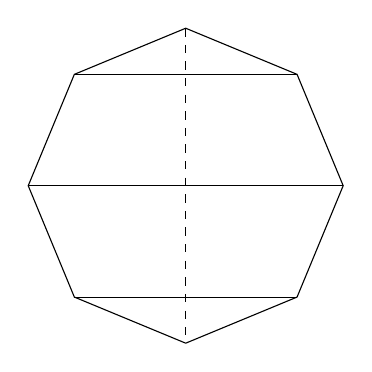
\begin{tikzpicture}[scale=2]
	\foreach \i in {0,1,4,5} {\coordinate (\i) at
		({cos(\i*45-45)},{sin(\i*45-45)});}
	\foreach \i in {2,3,6,7} {\coordinate (\i) at
		({cos(\i*45-45)},{sin(\i*45-45)});}
	\draw (7) \foreach \i in {0,...,7} {-- (\i)};
	\draw (0) -- (6) (1) -- (5) (2) -- (4);
	\draw[dashed] (3) -- (7);
	\end{tikzpicture}
	\caption{Расширение восьмиугольника в $\R^3$ (вид сверху), имеющее 6 гиперграней.}
	\label{fig:8gonEF}	
\end{figure}

Непосредственно из определений \ref{def:nonneg} и \ref{def:rect} следует, что число прямоугольного покрытия матрицы инциденций не превосходит неотрицательного ранга матрицы невязок.
Иными словами, справедлива следующая

\begin{theorem}[Яннакакис~\cite{Yannakakis:1988}]
	\label{thm:rcxc}
	$\xc(P) \ge \rc(P)$ для любого многогранника $P$.
\end{theorem}

Известно также, что нижние оценки в свойстве~\ref{prop:xc-base} верны и для числа прямоугольного покрытия.

\begin{property}[\cite{FioriniKPT:13}]\label{prop:rc-base}
	Пусть $P$ "--- выпуклый многогранник, $\face(P)$ "--- число всех его граней. Тогда \(\dim(P) + 1 \le \log_2 \face(P) \le \rc(P)\).
\end{property}

Кроме того, свойство~\ref{prop:xc-compare} при замене $\xc(\cdot)$ на $\rc(\cdot)$ тоже остается верным.
С~рядом других свойств числа прямоугольного покрытия матрицы инциденций гиперграней"=вершин многогранника можно ознакомиться в~\cite{FioriniKPT:13}.

Практически все известные в настоящее время нижние оценки сложности расширения многогранников получены с использованием теоремы~\ref{thm:rcxc} и (фактически комбинаторных) свойств \ref{prop:rc-base}, \ref{prop:xc-compare}.
Исключениями являются следующие три примера:
\begin{enumerate}
	\item Для многогранника паросочетаний $\Match(n)$ установлена экспоненциальная нижняя оценка сложности расширения~\cite{Rothvoss:2014}.
	При этом $\rc(\Match(n)) \in [n^2, n^4]$, согласно~\cite{FioriniKPT:13}.
	\item В~\cite{Fiorini:2012polygons} установлен факт существования $n$"~угольников, сложность расширения которых не меньше $\sqrt{2n}$, тогда как
	число прямоугольного покрытия матрицы инциденций $n$"~угольника находится в диапазоне от $\log_2 (2n)$ до $2\log_2 (2n)$ (как следует из~\cite{BenTal:2001, Fiorini:2012polygons}).
	\item Доказано существование семейств многогранников матроидов с экспоненциальной сложностью расширения~\cite{Rothvoss:2013} (в доказательстве используется тот факт, что число различных матроидов дважды экспоненциально относительно числа элементов множества"=носителя~\cite{Dukes:2003}). В то же время число прямоугольного покрытия для них не превышает квадрата от числа элементов множества"=носителя~\cite{Kaibel:2016}.
\end{enumerate}
Заметим, что задача о паросочетаниях является полиномиально разрешимой, а среди многоугольников и матроидов есть пимеры полиномиально разрешимых задач (например, оптимизация на вершинах правильного $n$"~угольника и оптимизация на матроиде остовных деревьев).
Таким образом, все известные факты говорят о том, что число прямоугольного покрытия матрицы инциденций вершин"=гиперграней многогранника дает весьма точную нижнюю оценку реальной сложности соответствующей оптимизационной задачи.
%(Исчерпывающее теоретическое обоснование этого феномена пока неизвестно.)



\section{Вопросы}
\label{sec:questions}

%{\color{red}Раздел сырой. Требует почти полной переделки!}

%Пусть $S = \{P(n)\}$ "--- некоторое семейство многогранников, каждый из которых представлен как выпуклая оболочка некоторого множества $X_n \subset \R^d$, $n\in\N$, $d = d(n)$. 
%С этим семейством связана оптимизационная задача OPT(S): дан номер $n\in\N$ и целевой вектор $\bm{c} \in \R^d$; требуется найти $\max \Set*{\bm{c}^T \bm{x} \given \bm{x} \in P(n)}$.

Как следует из перечисленных выше фактов, многогранники NP"~трудных задач во многих случаях обладают схожими свойствами. Например: NP"~полнота задачи распознавания несмежности вершин, небольшой диаметр графа, сверхполиномиальное кликовое число графа, сверхполиномиальные сложность расширения и число прямоугольного покрытия матрицы инциденций вершин"=гиперграней.
Часто эти сходства обусловлены тесными связями геометрического характера, обнаруживаемыми в разное время разными исследователями. 
Перечислим несколько известных примеров:
\begin{enumerate}
\item Булев квадратичный многогранник $\BQP(n)$ аффинно эквивалентен многограннику разрезов $\Cut(n-1)$~\cite[раздел~5.2]{Deza:2001}.
\item Многогранник совершенных паросочетаний $\Match(2n)$ есть проекция
некоторой грани многогранника задачи коммивояжера $\TSP(6n)$~\cite{Yannakakis:1991}.
\item Для каждого графа $G = (V,E)$ многогранник упаковок вершин $\Stable(G)$ является проекцией некоторой грани многогранника асимметричной задачи коммивояжера $\ATSP(n)$, где $n = |V| + 4|E|$~\cite{Yannakakis:1991}.
\item Многогранник $\ATSP(n)$ является гранью многогранника $\TSP(2n)$~\cite{Junger:1995TSP}.
\item Фиорини~\cite{Fiorini:2003} показал, что многогранники задачи о 3"~выполнимости и многогранники задачи о частичном упорядочивании являются гранями друг друга при надлежащем выборе кода многогранника (точные формулировки см. в разделе~\ref{subsec:k-Sat&POP}).
\item Авис и Тивари~\cite{AvisTiwary:2015} показали, что многогранник задачи о 3"~выполнимости является проекцией грани многогранника трехиндексной задачи о назначениях (подробнее "--- в разделе~\ref{sec:3Ass}).
\item Бучхейм, Вигеле и Женг~\cite{Buchheim:2010} показали, что многогранник квадратичной задачи линейного упорядочивания аффинно эквивалентен грани булева квадратичного многогранника (см. раздел~\ref{sec:QLOP}).
Аналогичный факт для многогранника квадратичной задачи о назначениях установлен независимо несколькими авторами~\cite{Rijal:1995, Kaibel:1997, Saito:2009}.
\end{enumerate}
В связи с этим естественными являются следующие вопросы общего характера. Можно ли систематически использовать такой способ сравнения для различных (других) семейств многогранников? 
Какие выводы на основе сравнений такого типа можно сделать в отношении различных комбинаторно"=геометрических характеристик многогранников?
Ответы на эти вопросы содержатся в главах \ref{chap:AffTheory}--\ref{chap:ExtAff}.

%В чем сходство между известными примерами комбинаторных семейств многогранников, для которых задача идентификации ребра NP"~трудна? Чем они отличаются от примеров, для которых эта задача полиномиально разрешима?

%Перечислим рассмотренные в этой главе характеристики многогранников: сложность идентификации грани (вершины, ребра, гиперграни), число вершин, число гиперграней, диаметр графа, кликовое число графа, сложность расширения, число прямоугольного покрытия матрицы инциденций вершин"=гиперграней.
Для каждой из рассмотренных в этой главе характеристик многогранников естественно задать следующий вопрос.
Есть ли связь между данной характеристикой и сложностью соответствующей оптимизационной задачи?
Кроме того, возникают вопросы более общего характера.
Какие известные в настоящее время комбинаторно"=геометрические характеристики  наиболее адекватно отражают реальную сложность соответствующей задачи?
Есть ли связь между комбинаторным типом многогранника и реальной сложностью задачи оптимизации на нем?
Исследованию этих проблем посвящены главы \ref{chap:Direct} и~\ref{chap:Counterexamples}.
